\section{Heatwave Application}

\begin{frame}{Motivation}

  \begin{columns}
    \begin{column}{0.6\linewidth}
      \begin{itemize}
        \item Measuring the effect of climate disasters
            \begin{itemize}
            \item Experimental approaches - if not unethical - are nearly impossible
            \item Researchers are stuck with observational data
            \item Recovering robust causal effects is critical policy input
            \end{itemize}
      \end{itemize}
    \end{column}
    \begin{column}{0.4\linewidth}
      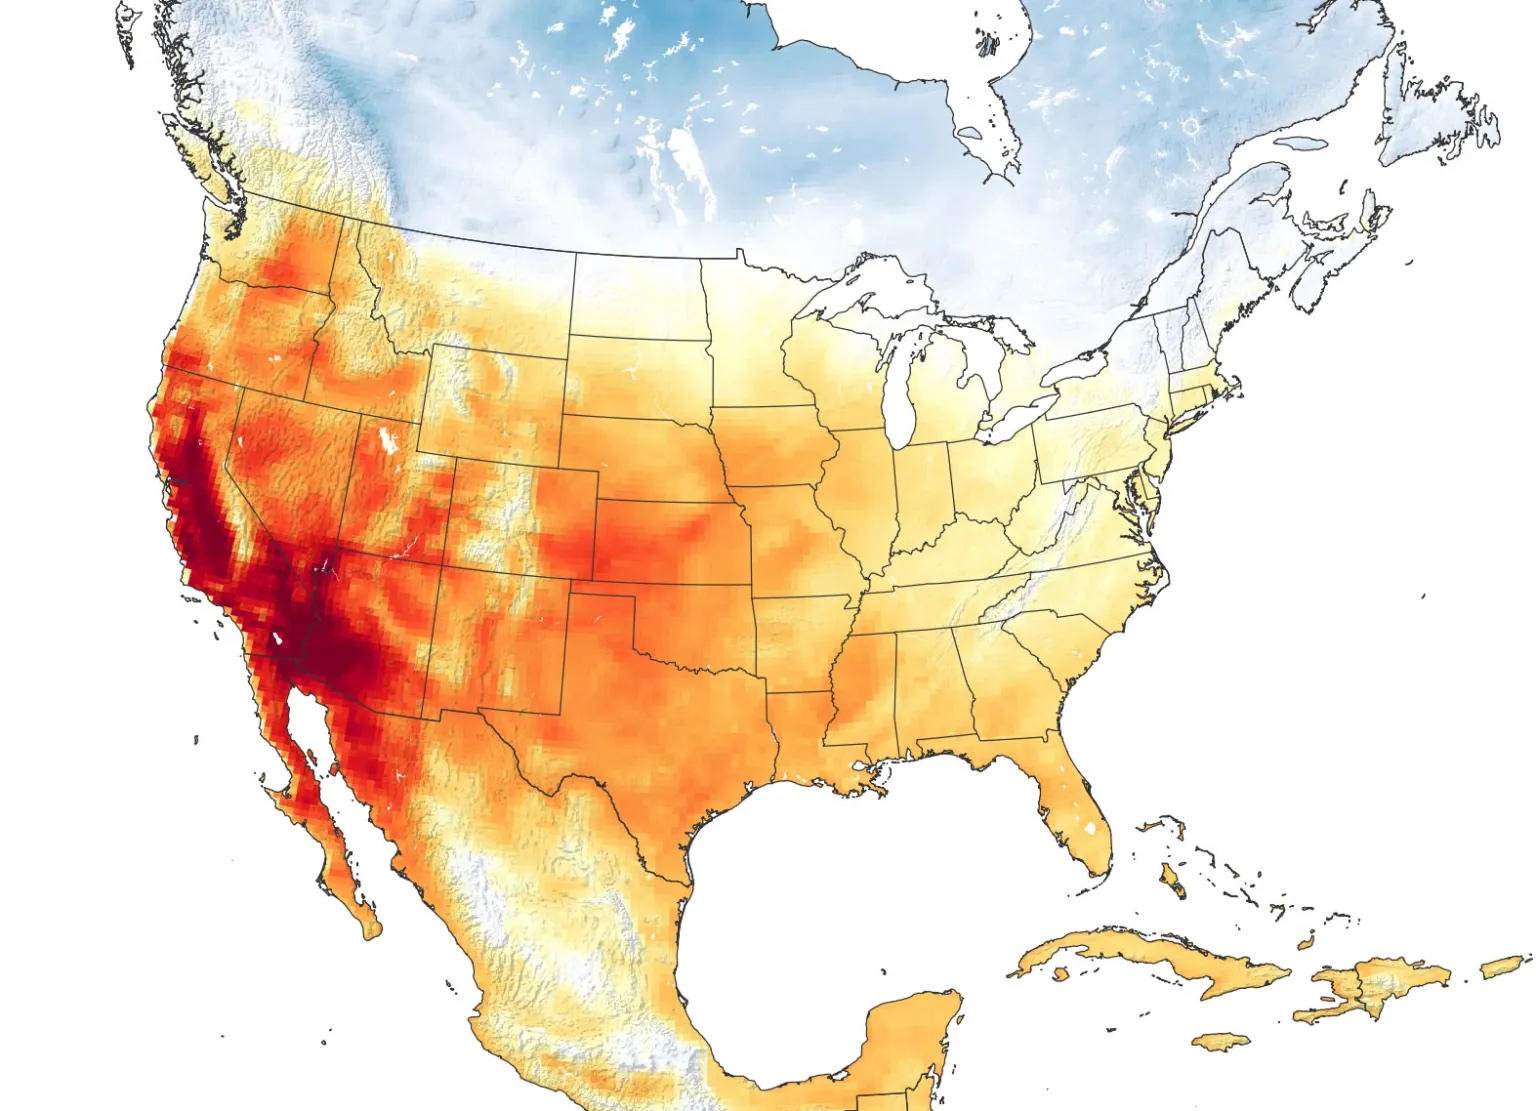
\includegraphics[scale=0.1]{figures/california-heatwave-2020-nasa-eo.jpeg}
      \caption{}
    \end{column}
  \end{columns}

\vspace{7pt}
\begin{center}
    \textbf{My Research Question: What is the effect of heat waves on hospitalization rates?}
\end{center}

  \note{
    This slide has notes too.
  }

\end{frame}

\begin{frame}{U.S. Cell Phone Ping Data}
Access to cell phone ping data: Unique opportunity to analyze spatial settings where units are not bound to spatial location.
\vspace{5pt}
\begin{columns}
    % Split 1
    \begin{column}{0.65\linewidth}
    \begin{itemize}
    \item Consider a densely populated area:
    \vspace{-7pt}
    \item Idea 1: Measure whether individuals visit hospitals via cell phone pings (Problem: Ping Irregularity)
    \vspace{-7pt}
    \item Idea 2: Measure the \textit{dispersion effect} of heat waves
    \end{itemize}
    \end{column}
    % Split 2
     \begin{column}{0.4\linewidth}
      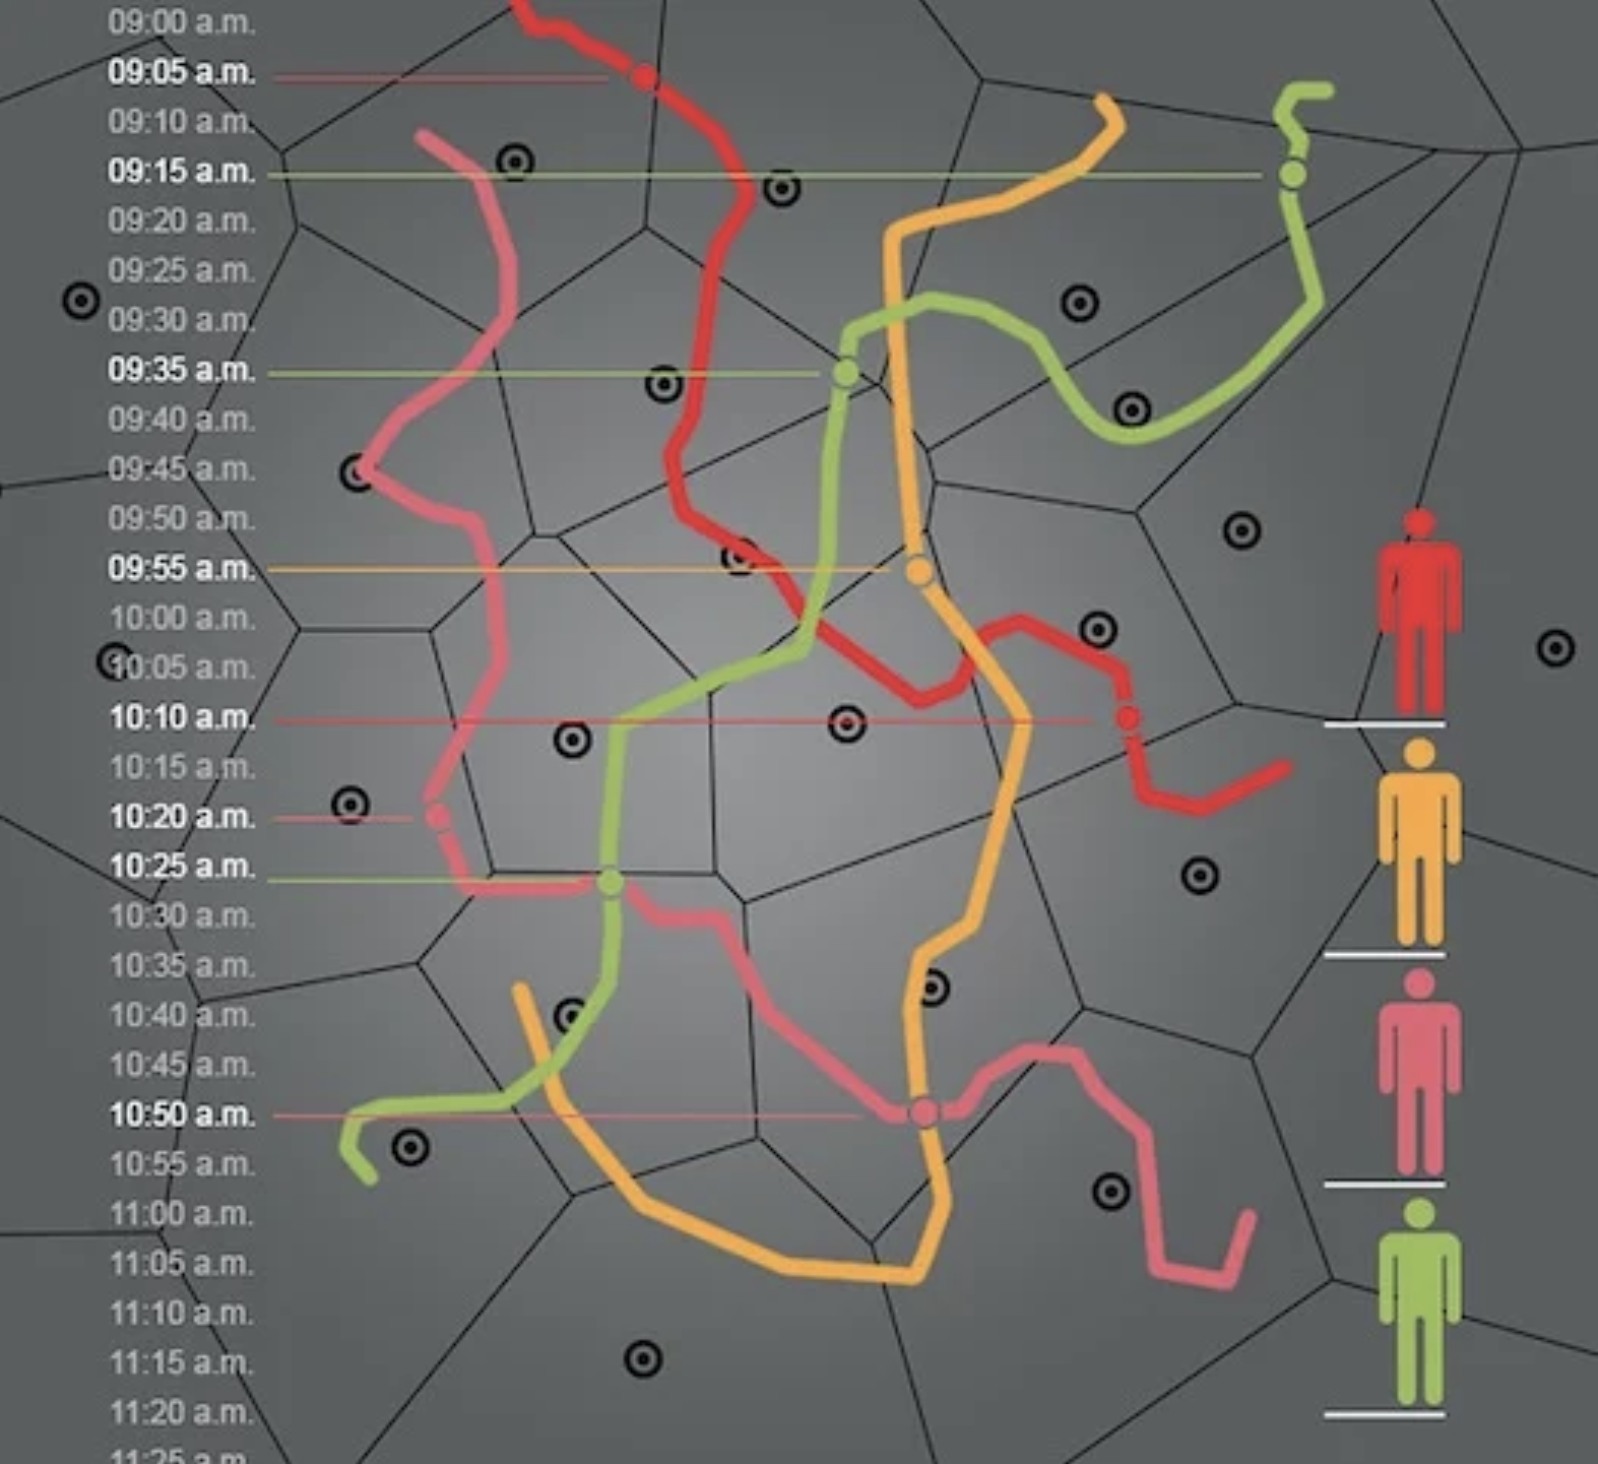
\includegraphics[scale=0.16]{figures/cell_ping.png}
      \caption{}
    \end{column}
\end{columns}
\end{frame}

\begin{frame}{Brainstorming}
- Think about mapping hospitals etc. 
- But also public facilities that are AC controlled??? These could be identified with the help of and conversations with community members and stewards
- Insight maybe: High-income - ppl just hunker down in their AC controlled places; low-income: Do people try to "escape"/ "flee" the heat to other places???
- classify/ define the concept of a "HEAT SHELTER" in addition to hospitals
- Define the median location of an individual as their home; also look into work location?
\end{frame}